
\documentclass[../../../interview-questions.tex]{subfiles}

\begin{document}

\subsection{Spring模块}

Spring 4的模块可参考\url{https://docs.spring.io/spring-framework/docs/4.0.x/spring-framework-reference/html/overview.html}。

\begin{enumerate}
    \item {Spring 核心容器}
Spring 核心容器 – 该层基本上是 Spring Framework 的核心。它包含以下模块:Spring Core/Spring Bean/SpEL (Spring Expression Language)/Spring Context
    \item{数据访问/集成}
数据访问/集成 – 该层提供与数据库交互的支持。它包含以下模块:JDBC (Java DataBase Connectivity)/ORM (Object Relational Mapping)/OXM (Object XML Mappers)/JMS (Java Messaging Service)/Transaction
\item{Web – 该层提供了创建 Web 应用程序的支持。}它包含以下模块:
Web
/Web – Servlet
/Web – Socket
/Web – Portlet
\item{AOP – 该层支持面向切面编程}
\item{Instrumentation – 该层为类检测和类加载器实现提供支持。}
\item{Test – 该层为使用 JUnit 和 TestNG 进行测试提供支持。}
几个杂项模块:
Messaging – 该模块为 STOMP 提供支持。它还支持注解编程模型,该模型用于从 WebSocket 客户端路由和处理 STOMP 消息。STOMP即Simple (or Streaming) Text Orientated Messaging Protocol,简单(流)文本定向消息协议,它提供了一个可互操作的连接格式,允许STOMP客户端与任意STOMP消息代理(Broker)进行交互。STOMP协议由于设计简单,易于开发客户端,因此在多种语言和多种平台上得到广泛地应用。

Aspects – 该模块为与 AspectJ 的集成提供支持。
\end{enumerate}

\begin{figure}[htbp]
	\centering
	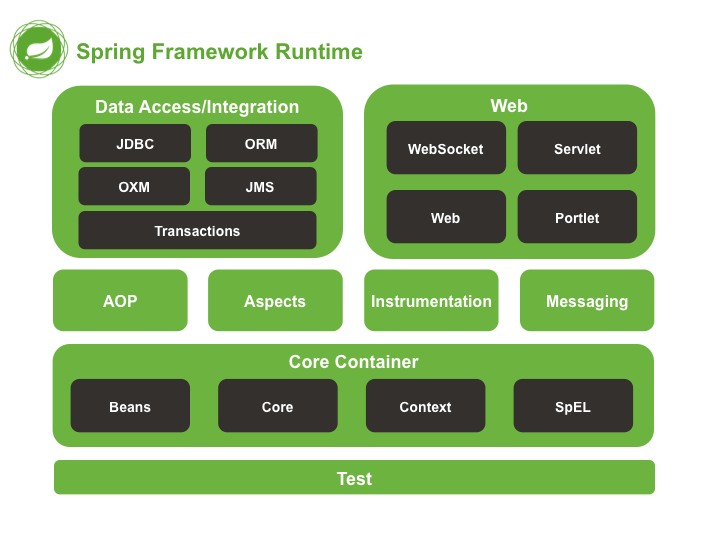
\includegraphics[scale=0.4]{spring-overview.png}
	\caption{Spring 4.0模块}
	\label{fig:springoverview}
\end{figure}


\end{document}
